%----------------------------------------------------------------------------------------
%	SECTION 1.1
%----------------------------------------------------------------------------------------

\section{The Metric Topology}

\begin{definition}
    A \textbf{metric} (or \textbf{distance function}) on a set $X$ is a map  $d:X \times X
    \rightarrow \R$ satisfying the following for all $x,y,z \in X$:
        \begin{enumerate}[label=(\arabic*)]
            \item $d(x,y) \geq 0$ and $d(x,y)=0$ if and only if $x=y$.

            \item $d(x,y)=d(y,x)$.

            \item (The Triangle Inequality) $d(x,y) \leq d(x,z)+d(z,y)$.
        \end{enumerate}
        We call $d(x,y)$ the \textbf{distance} between $x$ and  $y$, and given  $\epsilon>0$, we
    define the  \textbf{$\epsilon$-ball centered about $x$} to be the set $B_d(x,\epsilon)=\{y \in
    X: d(x,y)<\epsilon\}$.
\end{definition}

\begin{lemma}\label{2.2.1}
    Let $d$ be a metric on  $X$. For  $x,y \in X$, and  $B_d(x,\epsilon)$ an $\epsilon$-ball
    centered about  $x$, there is a  $\delta$-ball centered about  $y$,  $B_d(y,\delta)$ such that
    $B_d(y,\delta) \subseteq B_d(x,\epsilon)$.
\end{lemma}
\begin{proof}
    Let $y \in B_d(x,\epsilon)$ and let $\delta=\epsilon-d(x,y)$, and take $z \in B_d(y,\delta)$,
    then we have that $d(y,z)<\epsilon-d(x,y)$, thus $d(x,x) \leq d (x,y)+d(y,z)<\epsilon$ which
    complete the proof.
\end{proof}

\begin{theorem}\label{2.2.2}
    Let $d$ be a metric on  $X$. Then the colletion of all  $\epsilon$-balls about  $x$, for some
    $x \in X$ forms the basis for a topology on  $X$.
\end{theorem}
\begin{proof}
    Clearly $x \in B_d(x,\epsilon)$, by definition, so it remains to show that the intersection of
    two $\epsilon$-balls contains an  $\epsilon$-ball. Let  $B_1$ and $B_2$ be $\epsilon$-balls
    about  $x$, and let  $y \in B_1 \cap B_2$. By lemma \ref{2.2.1}, there are $\delta_1,\delta_2>0$
    such that $B_d(y,\delta_1) \subseteq B_1$ and $B_d(y,\delta_2) \subseteq B_2$. Now take
    $\delta=\min\{\delta_1, \delta_2\}$, then we see that $B_d(y,\delta) \subseteq B_1 \cap B_2$.
\end{proof}

\begin{definition}
    If $d$ is a metric on  $X$, we call the topology having as basis the collection of all
    $\epsilon$-balls centered about  $x$, for some  $x \in X$ and  $\epsilon>0$, the \textbf {metric
    topology} induced by $d$.		
\end{definition}

\begin{corollary}
    A set $U$ is open in the metric topology induced by  $d$ if and only if for each  $y \in U$, and
     $\delta>0$, there is a  $\delta$-ball centered about $y$ contained in  $U$.
\end{corollary}

\begin{figure}[h]
    \centering
    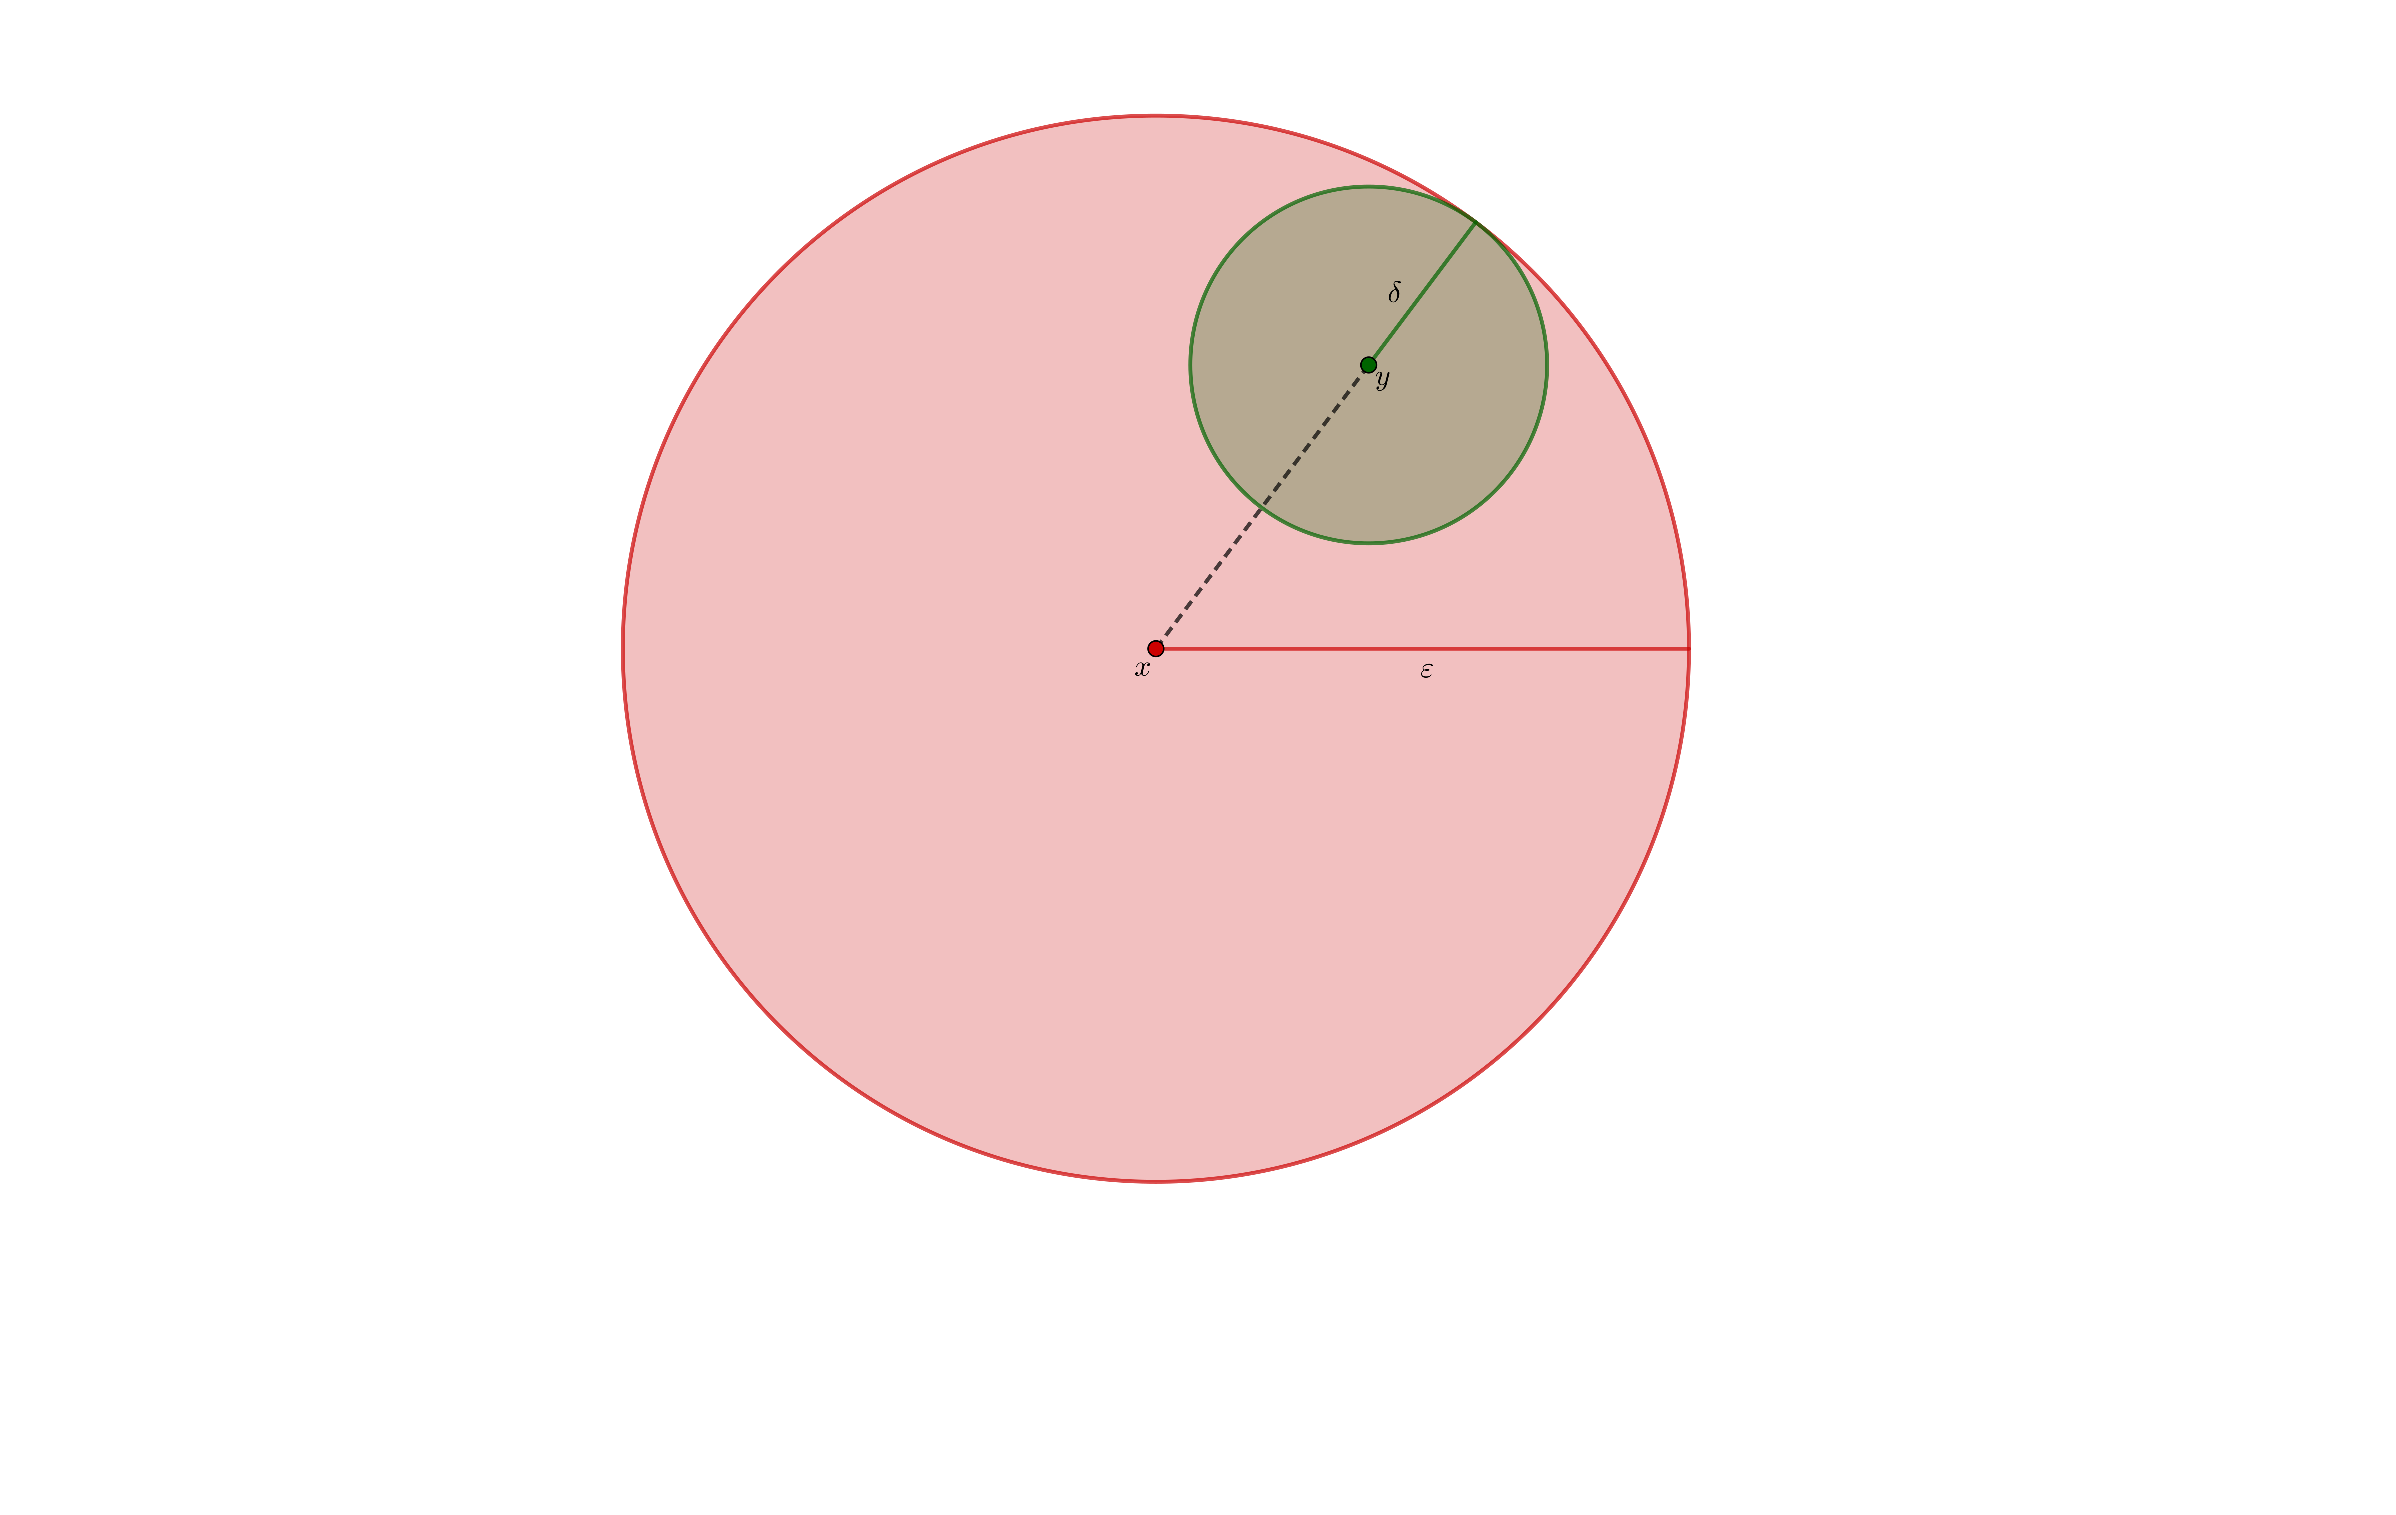
\includegraphics[scale = 0.2]{Figures/Chapter2/openBall.eps}
    \caption{All $\epsilon$-balls centered about  $x$ are open in the metric topology by lemma
    \ref{2.2.1}.}
    \label{fig2.1}
\end{figure}

\begin{example}
    \begin{enumerate}[label=(\arabic*)]
        \item Define $d(x,y)=1$ if $x \neq y$ and  $d(x,y)=0$ if $x=y$. Clearly  $d$ is a metric on
            $X$, and induces the discrete topology on  $X$. The basis  $B_d(x,1)=\{x\}$

        \item The standard metric on $\R$ is defined to be  $d(x,y)=|x-y|$ and is a metric on $\R$ 
            (that is, the absolute $|cdot|$ is a metric on  $\R$). This metric induces the standard
            topology on $\R$ as we see that it has basis $B_d(x,\epsilon)=\{y \in \R:
            |x-y|<\epsilon\}=\{y \in \R: y-\epsilon<x<y+\epsilon\}=(y-\epsilon,y+\epsilon)$.
    \end{enumerate}		
\end{example} 

\begin{definition}
    If $X$ is a topological space, we call  $X$ \textbf {metrizable} if there is a metric $d$ which
    induces the topology on $X$. A \textbf {metric space} is a metrizable space $X$ together with
    the metric inducing the topology of $X$.
\end{definition}

\begin{definition}
    Let $X$ be a metric space with metric $d$. A subset $A \subseteq X$ is said to be \textbf
    {bounded} if there is an $M>0$ such that $d(a_1,a_2) \leq M$ for all $ a_1,a_2 \in X$. We define
    the \textbf{diameter} of a bounded set $A$ to be $\diam{A}=\sup\{d(a_1,a_2):a_1,a_2 \in A\}$.
\end{definition}

It is easy to see that boundedness of a set does not depend on the topology of $X$, but on the
metric.

\begin{theorem}\label{2.2.3}
    Let $X$ be a metric space with metric $d$ and define  $\bar{d}:X \times X \rightarrow \R$ by
    $\bar{d}=\min\{d(x,y),1\}$ for all $x,y \in X$. Then  $\bar{d}$ is a metric on $X$ that induces
    the same topology as  $d$.
\end{theorem}
\begin{proof}
    Clearly we have that $0 \leq \bar{d}(x,y) \leq 1$, and that
    $\bar{d}(x,y)=\min\{d(x,y),1\}=\min\{d(y,x),1\}=\bar{d}(y,x)$. It remains to show the triangly
    inequality.

    Now if $d(x,z) \leq 1$ and $d(z,y) \leq 1$, then by the triangle inequality $d(x,y) \leq 1$ and
    $\bar{d}(x,y) \leq \bar{d}(x,z)+\bar{d}(z,y)$. Now if $d(x,z)<1$ and $d(z,y)<1$, we get the same
    conclusion. Thus we see that $\bar{d}$ is a metric on $X$.

    Now take as basis the collection of all  $\epsilon$-balls with  $0<\epsilon<1$, and any basis
    element of  $x$ contains such an  $\epsilon$-ball, thus  $\bar{d}$ induces the same topology as
    $d$.
\end{proof}

\begin{definition}
    We call $\bar{d}$ the \textbf{standard bounded metric} corresponding to $d$.		
\end{definition}

\begin{definition}
    Let $x \in \R^n$. We define the \textbf {norm} of $x$,  $||x||$, to be
    $||x||=\sqrt{x_1^2+ \dots +x_n^2}$. We define the \textbf{square metric} $\rho$  on 
    $\R^n$ to be  $\rho(x,y)=\mac\{|x_1-y_1|, \dots |x_n-y_n|\}$.
\end{definition}

Before we show that $||\cdot||$ and  $\rho$ are metrics, we introduce the following:

 \begin{definition}
    Let $x,y \in \R^n$. We define the \textbf{inner product} of $x$ and $y$ to be:
        \begin{equation}
            \vbrack{x,y}=x_1y_1+ \dots x_ny_n
        \end{equation}
\end{definition}

\begin{lemma}\label{2.2.4}
    For $x,y \in \R^n$,  $\vbrack{x,y+z}=\vbrack{x,y}+\vbrack{x,z}$ and $|\vbrack{x,y}| \leq
    ||x||||y||$.
\end{lemma}
\begin{proof}
    W have $\vbrack{x,y+z}=x_1(y_1+z_1)+ \dots +x_n(y_n+z_n)=(x_1y_1 + \dots +x_n_y_n)+(x_1z_1+
    \dots +x_nz_n)=\vbrack{x,y}+\vbrack{x,z}$.

    Now if $x=0$ and  $y=0$, then  $|\vbrack{x,y}|=||x||||y||=0$, so suppose that both $x,y \neq 0$,
    and let  $a=\frac{1}{||x||}$ and $b=\frac{1}{||y||}$. Notice that $||ax+by|| \geq 0$ and
    $||ax-by|| \geq 0$, then $||ax+by||^2||ax-by||^2=||x||^2||y^2||-|\vbrack{x,y}|^2\geq 0$, hence 
    $|\vbrack{x,y}| \leq ||x||||y||$.
\end{proof}
\begin{remark}
    We call the last relation in the lemma the \textbf{Cauchy-Schwarz inequality}.
\end{remark}

\begin{theorem}\label{2.2.5}
    Both the norm and square metrics make  $\R^n$ into a metric space.
\end{theorem}
\begin{proof}
    We start with the norm. Now clearly, since $\sqrt{x} \geq 0$ (for real numbers), $||x-y|| \geq
    0$, and  if $||x-y||=0$ then  $(x_1-y_1)^2+ \dots (x_n-y_n)^2=0$ hence $x_i=y_i$ for all  $1
    \leq i \leq n$, and if  $x_i=y_i$, then clearly  $||x-y||=0$. We also see that
    $||x-y||=||y-x||$.

    Now consider  $z \in \R^n$, notice that
    $||x+y||^2=\vbrack{x+y,x+y}=\vbrack{x+y,x}+\vbrack{x+y,y}=\vbrack{x,x}+\vbrack{y,y} \leq
    ||x||^2+||y||^2$. Using this we have $||x-z||+||z-y|| \geq ||x-y||$ (square the left hand side
    and evaluate), so  $||\cdot||$ is a metric on  $\R^n$.

    Now consider the square metric. Clearly we have that $\rho(x,y) \geq 0$ and that $\rho(x,y)=0$
    if and only if $x=y$  (snce $|\cdot|$ is also a metric), we also see that $\rho(x,y)=\rho(y,x)$.

    Now let $x \in \R^n$, and we have for all  $1 \leq i \leq n$ that  $|x_i-y_i| \leq
    |x_i-z_i|+|z_i-y_i|$, hence by definition $|x_i-y_i| \leq  \rho(x,z)+\rho(z,y)$, thus $\rho(x,y)
    \leq \rho(x,z)+\rho(z,y)$ and $\rho$ is a metric.
\end{proof}

\begin{lemma}\label{2.2.6}
    Let $d$ and  $d'$ be metrics on  $X$ and let  $\Tc$ and  $\Tc'$ be the topologies induced by
    $d$ and  $d'$ respectively.  $\Tc \subseteq \Tc'$ if and only if for each  $x \in X$, and
    $\epsilon>0$, there is a  $\delta>0$ such that  $B_{d'}(x,\epsilon) \subseteq B_d(x,\epsilon)$.
\end{lemma}
\begin{proof}
    Suppose that $\Tc \subseteq \Tc'$, and take  $B_d(x,\epsilon)$ in $\Tc$, then by lemma \ref
    {2.2.1}, there is a $B'$ in  $\Tc'$ or which  $B' \subseteq B_d(x,\epsilon)$, hence there is a
    $\delta$-ball about $x$ for which  $B_{d'}(x,\delta) \subseteq B'$.

    Conversly, suppose for $x \in X$ and  $\epsilon>0$, that ther is a $\delta>0$ for which
    $B_{d'}(x,\delta) \subseteq B_d(x,\epsilon)$. Given a basis $B$ of  $\Tc$, ther is an
    $\epsilon$-ball about  $x$ contained in  $B$, hence  $B_d(x,\epsilon)$ is also in $B$, thus we
    have that  $\Tc \subseteq \Tc'$.
\end{proof}

\begin{theorem}\label{2.2.7}
    The norm and the square metric both induce the product topology on $\R^n$.
\end{theorem}
\begin{proof}
    Notics that $\rho(x,y) \leq ||x-y|| \leq \sqrt{n}\rho(x,y)$. This first inequality shows that
    $B_{||\cdot||}(x,\epsilon) \subseteq B_{\rho}(x,\epsilon)$, and the second shows that
    $B_{\rho}(x,\frac{\epsilon}{\sqrt{n}}) \subseteq B_{||\cdot||}(x,\epsilon)$, thus both
    $||\cdot||$ and  $\rho$ induce the same topology.

    Now let  $B=(a_1,b_1) \times \dots \times (a_n,b_n)$ be a basis for the product topology on $
    \R^n$. Since, for each  $i$, there is an  $\epsilon_i>0$ such that
    $(x_i-\epsilon_i,x_i+epsilon_i) \subseteq (a_i,b_i)$, choosing $\epsilon=\min\{\epsilon_1,
    \dots, \epsilon_n\}$, we see that $B_{\rho}(x,\epsilon) \subseteq B$. Conversely, given $y \in
    B_{\rho}(x,\epsilon)$, notice that $B_{\rho}(x, \epsilon)=(x_1-\epsilon,x_1+\epsilon) \times
    \dots \times (x_n-\epsilon,x_n+\epsilon)$, thus $B \subseteq B_{\rho}(x,\epsilon)$. Thus the
    topologies are the same.
\end{proof}

\begin{definition}
    Given an index set $J$ and given points  $x=(x_{\alpha})$ and $y=(y_{\alpha})$ fo $\R^J$, we
    define the \textbf {uniform metric} $\bar{\rho}$ on $\R^J$ by
    $\bar{\rho}(x,y)=\sup\{\bar{d}(x_{\alpha},y_{\alpha}): \alpha \in J\}$, where $\bar{d}$ is the
    standard bounded metric on  $\R^J$. We call the topology induced by $\bar{\rho}$ the
    \textbf{uniform topology}.
\end{definition}

\begin{theorem}\label{2.2.8}
    The uniform topology on $\R^J$ is finer than the product topology on  $\R^J$ and coarser than
    the box topology on  $\R^J$, and all three topologies are different if  $J$ is infinite.
\end{theorem}
\begin{proof}
    Let $x=(x_[\alpha])$ and $\prod{U_{\alpha}}$ be a basis element for the product topology, and
    let $\alpha_1 ,\dots, \alpha_n$ be the indices for which $U_{\alpha} \neq \R$, and for each $i$,
    choose  $\epsilon_i>0$ such that the  $\epsilon_i$-ball about  $x_{\alpha_i}$,
    $B_{\bar{d}}(x_{\alpha_i},\epsilon_i) \subseteq U_{\alpha}$. Let $\epsilon=\min\{\epsilon_1,
    \dots, \epsilon_n\}$, and let $z=(z_{\alpha}) \in \R^J$ be such that $\bar{\rho}(x,z)<\epsilon$.
    Then $\bar{d}(x_{\alpha},z_{\alpha})<\epsilon$ for all $\alpha$. Hence  $B_{\bar{\rho}}
    \subseteq \prod{U_{\alpha}}$ for all $\alpha$; so the uniform topology is finer.

    Likewise, consider $B$ the $\epsilon$-ball about  $x$ in the  $\bar{\rho}$ metric. Then the box
    $U=\prod{(x_{\alpha}-\frac{\epsilon}{2},x_{\alpha}+\frac{\epsilon}{2})}$ and $y \in U$ if
    $\bar{d}(x_{\alpha},y_{\alpha}<\frac{\epsilon}{2})$, then $\bar {\rho}(x,y) \leq
    \frac{\epsilon}{2}$, so $U \subseteq B$, and the uniform topology is coarser.

    Now in the case where  $J$ is infinite, if  $J$ is uncountable, we are done, since there is no
    way to map the indices of  $J$ onto  $\Z^+$. So consider the case where  $J$ is countable, and
    map  $J \rightarrow \Z^+$ by  $\alpha_i \rightarrow i$. Let
    $U=\prod{(x_i-\epsilon,x_i+\epsilon)}$ and consider a base $B_{\bar{\rho}}(x,\epsilon)$. We have
    that for  $y \in B_{\bar{\rho}}(x,\epsilon)$ that
    $\bar{d(x_{\alpha},y_{\alpha})}=\min\{\rho(x_i,y_i),1\}$, we have that
    $\bar{d}(x_i,y_i)=\bar{\rho}(x_i,y_i)$ or $1$, and if we choose  $0<\epsilon<1$, then
    $\bar{\rho}$ fails to put $B_{\bar{\rho}}(x,\epsilon)$ inside of $U$. Likewise, the basis
    $\prod{U_{\alpha}}$ (in the prodct topology) failes to be contained in
    $B_{\bar{\rho}}(x,\epsilon)$ by the same argument. Thus the uniform topology is not necessarily finer than
    the box topology, nor coarser than the product topology in $\R^J$, when $J$ is infinite.
\end{proof}
\begin{remark}
    Clearly the box, product and uniform topologies on $\R^J$ are the same when  $J$ is finite, as
    the box and product topologies are the same for finite product spaces.
\end{remark}

\begin{theorem}\label{2.2.9}
    Let $\bar{d}(a,b)=\min{|a-b|,1\}$ be the standard bounded metric on $\R$, and for  $x,y \in
    \R^{\omega}$, define:
        \begin{equation}
            D(x,y)=\sup\{\frac{\bar{d}(x_i,y_i)}{i}\}
        \end{equation}.
    Then $D$ is a metric that induces the product topology on $\R^{\omega}$.
\$B_{\bar{\rho}}(x,\epsilon)$
\end{theorem}
\begin{proof}
    Since $\bar{d}$ is a metric, $D$ satisfies the conditions for a metric space, it is worth
    looking into the case for the triangle inequality however. Notice that for all  $i$,  $
    \frac{\bar{d}(x_i,y_i)}{i} \leq \frac{\bar{d}(x_i,z_i)}{i}+\frac{\bar{d}(z_i,y_i)}{i} \leq
    D(x,z)+D(z,y)$, thus $D(x,y) \leq D(x,z)+D(z,y)$.

    Now let $U$ be open in the metric topology induced by  $D$ and let  $x \in U$. Choose an
    $\epsilon$-ball  $B_D(x,\epsilon) \subseteq U$, and choose $N>0$ large enough that  $
    \frac{1}{N}<\epsilon$, and let $V=(x_1-\epsilon,x_1+\epsilon) \times \dots \times
    (x_N-\epsilon,x_N+\epsilon) \times \R \times \dots \times \R \times \dots$. Given $y \in
    \R^{\omega}$, we have $ \frac{\bar{d}(x_i,y_i)}{i} \leq \frac{1}{N}$, thus $D(x,y)$ \leq
    \max\{\bar(d)(x_1,y_1),\dots, \bar(d)(x_i,y_i)}{i}, \frac{1}{N}\} for all $i \geq N$. Now if  $y
    \in V$, then the expression is less than  $\epsilon$, so  $V \subseteq B_D(x,\epsilon)$.
    Convsersely, let $U=\prod{U_{i}}$ with $U_i$ open in  $\R$ for  $i=\alpha_1, \dots, \alpha_n$,
    and $U_i=\R$ for all other  indices. Given $x \in U$, for  $i=\alpha_1, \dots, \alpha_n$ and let
    $\epsilon=\min\{\frac{\epsilon_i}{i}:i=\alpha_1, \dots, \alpha_n\}$. Letting $B_d(x,\epsilon)$,
    we see that $ \frac{\bar{d}(x_i,y_i)}{i} \leq D(x,y)<\epsilon$. Now if $i=\alpha_1, \dots,
    \alphaalpha_n$, then $\bar{d}(x_i,y_i)<\epsilon_i \leq 1$, hence $|x_i-y_i|<\epsilon_i$, thus
    $y \in U$.
\end{proof}
